\subsection{Alloy Specification}
Here is the Alloy specification of the system described in the RASD:

\vspace{0.5cm}
\lstset{language=alloy, basicstyle=\ttfamily\footnotesize, breaklines=true}
\begin{lstlisting}
// ---------- Core Signatures ----------

abstract sig User {
	id: one ID,
	email: one ID,
	name: one ID,
	phoneNumber: one ID
}

// A student user who has a CV and can submit internship applications.
sig Student extends User {
	cv: one CV,
	applications: set Application
} {
	// Every student must have a CV.
	some cv
}

// A company user that offers internships.
sig Company extends User {
	companyName: one ID,
	industry: one ID,
	internships: set Internship // Internships provided by the company.
}

// A university user managing students and handling complaints.
sig University extends User {
	universityName: one ID,
	students: set Student, // The students enrolled in the university.
	complaints: set Complaint // Complaints registered with the university.
}

// A CV containing a summary, skills, education, and experience details.
sig CV {
	skills: set Skill,
	education: set Education,
	experience: set Experience,
	summary: one ID
}

// An internship with specific details such as title, description, requirements, and dates.
sig Internship {
	title: one ID,
	description: one ID,
	requirements: set Skill, // Skills required for the internship.
	startDate: one Date,
	endDate: one Date,
	status: one Status
}

// An application linking a student to an internship.
sig Application {
	student: one Student,
	internship: one Internship,
	applicationDate: one Date,
	status: one Status
}

// An interview scheduled for a specific application.
sig Interview {
	application: one Application,
	scheduledTime: one DateTime, // Time slot for the interview.
	status: one Status,
	feedback: lone ID
}

// A complaint filed by a user with a description and status.
sig Complaint {
	id: one ID,
	description: one ID, // Complaint details.
	status: one Status,
	filingDate: one Date,
	complainant: one User // The user who raised the complaint.
}

// Represents textual identifiers for various elements.
sig ID {}

// ---------- Enumerations ----------

enum Skill  	{ JAVA, PYTHON, CPP, JAVASCRIPT, DATABASE }
enum Education  { BACHELORS, MASTERS, PHD }
enum Experience { JUNIOR, MID, SENIOR }
enum Status 	{ OPEN, CLOSED, PENDING, APPROVED, REJECTED }
enum DateTime   { MORNING, AFTERNOON, EVENING }

// Represents months as a hierarchy rather than an enumeration.
abstract sig Date {}
one sig JAN, FEB, MAR, APR, MAY, JUN, JUL, AUG, SEP, OCT, NOV, DEC extends Date {}

// ---------- Utility Function + Predicate ----------

// Assigns a numerical index to each month for easy comparison.
fun dateIndex[d: Date]: Int {
	d = JAN => 1
	else d = FEB => 2
	else d = MAR => 3
	else d = APR => 4
	else d = MAY => 5
	else d = JUN => 6
	else d = JUL => 7
	else d = AUG => 8
	else d = SEP => 9
	else d = OCT => 10
	else d = NOV => 11
	else 12
}

// Validates that one date comes before another.
pred dateOrder[d1, d2: Date] {
	dateIndex[d1] < dateIndex[d2]
}

// ---------- Facts & Constraints ----------

// Enforces unique IDs for all users.
fact UserIDsAreUnique {
	all disj u1, u2: User | u1.id != u2.id
}

// Ensures the system always contains at least one student, company, and university.
fact AtLeastOneOfEach {
	some Student
	some Company
	some University
}

// Every student must be associated with exactly one university.
fact StudentUniversityRelationship {
	all s: Student | one u: University | s in u.students
}

// Ensures internships are owned by exactly one company.
fact InternshipOwnership {
	all i: Internship | one c: Company | i in c.internships
}

// Ensures internships have a valid time frame, with the start date before the end date.
fact InternshipDates {
	all i: Internship | dateOrder[i.startDate, i.endDate]
}

// A student can only apply for internships where their CV covers all required skills.
fact ValidApplications {
	all a: Application |
    	a.internship.requirements in a.student.cv.skills
}

// Guarantees that open internships have at least one applicant.
fact OpenInternshipsMustHaveApplicants {
	all i: Internship |
    	i.status = OPEN implies some a: Application | a.internship = i
}

// Prevents duplicate applications for the same internship by the same student.
fact UniqueApplications {
	all disj a1, a2: Application |
    	(a1.student != a2.student) or (a1.internship != a2.internship)
}

// If an application is approved, the corresponding internship cannot remain open.
fact ApprovedApplicationClosesInternship {
	all a: Application |
    	a.status = APPROVED implies a.internship.status != OPEN
}

// Ensures interviews are only scheduled if the student's skills meet the internship requirements.
fact ValidInterview {
	all i: Interview |
    	i.application.student.cv.skills in i.application.internship.requirements
}

// Complaints (if not rejected) must have a valid complainant.
fact ComplaintResolution {
	all c: Complaint |
    	c.status != REJECTED implies some c.complainant
}

// Ensures all complaints have unique IDs and exactly one complainant.
fact ValidComplaints {
	all c: Complaint | one u: User | c.complainant = u
	all disj c1, c2: Complaint | c1.id != c2.id
}

// Suggests that students whose skills match the requirements of an internship should apply.
fact RecommendedApplications {
	all s: Student, i: Internship |
  	(i.requirements in s.cv.skills) implies
    	(some a: Application | a.student = s and a.internship = i)
}

// ---------- Simple Run Command ----------

// Generates an instance of the model up to a scope of 5.
run {} for 5

// ---------- Analysis Code (Assertions + Predicates) ----------

// Assertion: Prevents students from applying to the same internship multiple times.
assert UniqueApplicationsAssert {
	all disj a1, a2: Application |
    	a1.student = a2.student and a1.internship = a2.internship
    	implies a1 = a2
}
check UniqueApplicationsAssert for 5

// Assertion: Validates that open internships have at least one applicant.
assert OpenInternshipsAssert {
	all i: Internship |
    	i.status = OPEN implies some a: Application | a.internship = i
}
check OpenInternshipsAssert for 5

// Assertion: Ensures students are only interviewed if they meet the requirements.
assert ValidInterviewAssert {
	all i: Interview |
    	i.application.student.cv.skills in i.application.internship.requirements
}
check ValidInterviewAssert for 5

// Assertion: Complaints (if not rejected) must have valid complainants.
assert ComplaintResolutionAssert {
	all c: Complaint |
    	c.status != REJECTED implies some c.complainant
}
check ComplaintResolutionAssert for 5

// Assertion: Approved applications mean the internship is not open anymore.
assert ApprovedApplicationClosesInternshipAssert {
	all a: Application |
    	a.status = APPROVED implies a.internship.status != OPEN
}
check ApprovedApplicationClosesInternshipAssert for 5

// Assertion: If a student meets all required skills, an application should exist.
assert RecommendedApplicationsAssert {
	all s: Student, i: Internship |
  	(i.requirements in s.cv.skills) implies
    	(some a: Application | a.student = s and a.internship = i)
}
check RecommendedApplicationsAssert for 5

//------------------------------------------------------
//  Scenarios to RUN and visualize
//------------------------------------------------------

/**
 * Scenario: A student is applying for an internship.
 * The internship is open, and the student has the required skills for it.
 * We also ensure that the application is properly linked to both the student
 * and the internship.
 */
pred StudentAppliesToOpenInternship {
	some s: Student, i: Internship |
    	i.status = OPEN
    	and i.requirements in s.cv.skills
    	and some a: Application | a.student = s and a.internship = i
}
/** Execute this scenario with up to 5 instances */
run StudentAppliesToOpenInternship for 5

/**
 * Scenario: An internship gets approved for a student.
 * Once approved, the internship is no longer open for applications.
 * This helps verify that the status transitions are consistent.
 */
pred ApprovedInternshipScenario {
	some a: Application |
    	a.status = APPROVED
    	and a.internship.status != OPEN
}
/** Execute this scenario with up to 5 instances */
run ApprovedInternshipScenario for 5

/**
 * Scenario: A complaint has been submitted and isn't rejected.
 * If the complaint is still under consideration or resolved,
 * we need to ensure there’s a valid complainant tied to it.
 */
pred ValidComplaintScenario {
	some c: Complaint |
    	c.status != REJECTED
}
/** Execute this scenario with up to 5 instances */
run ValidComplaintScenario for 5

\end{lstlisting}

\vspace{0.5cm}

\subsection{Alloy Analysis Results}

The Alloy Analyzer was used to validate the constraints, assertions, and facts defined in the model. The following results were obtained:

%-----------------------------------------
\subsubsection{Assertion 1: UniqueApplicationsAssert}
\paragraph{Description:} This assertion ensures that no student can apply to the same internship more than once.
\paragraph{Check Command:}
\begin{verbatim}
check UniqueApplicationsAssert for 5
\end{verbatim}
\paragraph{Result:} 
\begin{verbatim}
Executing "Check UniqueApplicationsAssert for 5"
   Solver=sat4j Bitwidth=4 MaxSeq=5 SkolemDepth=1 Symmetry=20 Mode=batch
   11978 vars. 1040 primary vars. 22948 clauses. 22ms.
   No counterexample found. Assertion may be valid. 3ms.
\end{verbatim}

%-----------------------------------------
\subsubsection{Assertion 2: OpenInternshipsAssert}
\paragraph{Description:} Ensures that all internships marked as \texttt{OPEN} have at least one associated applicant.
\paragraph{Check Command:}
\begin{verbatim}
check OpenInternshipsAssert for 5
\end{verbatim}
\paragraph{Result:} 
\begin{verbatim}
Executing "Check OpenInternshipsAssert for 5"
   Solver=sat4j Bitwidth=4 MaxSeq=5 SkolemDepth=1 Symmetry=20 Mode=batch
   11958 vars. 1035 primary vars. 22710 clauses. 23ms.
   No counterexample found. Assertion may be valid. 4ms.
\end{verbatim}

%-----------------------------------------
\subsubsection{Assertion 3: ValidInterviewAssert}
\paragraph{Description:} Validates that students are only interviewed if their skills match the internship requirements.
\paragraph{Check Command:}
\begin{verbatim}
check ValidInterviewAssert for 5
\end{verbatim}
\paragraph{Result:} 
\begin{verbatim}
Executing "Check ValidInterviewAssert for 5"
   Solver=sat4j Bitwidth=4 MaxSeq=5 SkolemDepth=1 Symmetry=20 Mode=batch
   12040 vars. 1035 primary vars. 22907 clauses. 23ms.
   No counterexample found. Assertion may be valid. 49ms.
\end{verbatim}

%-----------------------------------------
\subsubsection{Assertion 4: ComplaintResolutionAssert}
\paragraph{Description:} Ensures that all complaints not marked \texttt{REJECTED} have valid complainants.
\paragraph{Check Command:}
\begin{verbatim}
check ComplaintResolutionAssert for 5
\end{verbatim}
\paragraph{Result:} 
\begin{verbatim}
Executing "Check ComplaintResolutionAssert for 5"
   Solver=sat4j Bitwidth=4 MaxSeq=5 SkolemDepth=1 Symmetry=20 Mode=batch
   11918 vars. 1035 primary vars. 22639 clauses. 23ms.
   No counterexample found. Assertion may be valid. 3ms.
\end{verbatim}

%-----------------------------------------
\subsubsection{Assertion 5: ApprovedApplicationClosesInternshipAssert}
\paragraph{Description:} Ensures that once an application is \texttt{APPROVED}, the associated internship is no longer \texttt{OPEN}.
\paragraph{Check Command:}
\begin{verbatim}
check ApprovedApplicationClosesInternshipAssert for 5
\end{verbatim}
\paragraph{Result:} Verified. The model enforces that \texttt{APPROVED} 
\begin{verbatim}
Executing "Check ApprovedApplicationClosesInternshipAssert for 5"
   Solver=sat4j Bitwidth=4 MaxSeq=5 SkolemDepth=1 Symmetry=20 Mode=batch
   11949 vars. 1035 primary vars. 22747 clauses. 25ms.
   No counterexample found. Assertion may be valid. 2ms.
\end{verbatim}
%-----------------------------------------
\subsubsection{Assertion 6: RecommendedApplicationsAssert}
\paragraph{Description:} If a student’s skills match an internship’s requirements, an application should exist.
\paragraph{Check Command:}
\begin{verbatim}
check RecommendedApplicationsAssert for 5
\end{verbatim}
\paragraph{Result:} 
\begin{verbatim}
Executing "Check RecommendedApplicationsAssert for 5"
   Solver=sat4j Bitwidth=4 MaxSeq=5 SkolemDepth=1 Symmetry=20 Mode=batch
   12128 vars. 1040 primary vars. 23002 clauses. 23ms.
   No counterexample found. Assertion may be valid. 7ms.
\end{verbatim}

%-----------------------------------------
\subsubsection{Scenario: Student Applies to an Open Internship}
\paragraph{Description:} A scenario where a student with matching skills applies to an \texttt{OPEN} internship.
\paragraph{Predicate:}
\begin{verbatim}
pred StudentAppliesToOpenInternship {
    some s: Student, i: Internship |
        i.status = OPEN
        and i.requirements in s.cv.skills
        and some a: Application |
            a.student = s and a.internship = i
}
run StudentAppliesToOpenInternship for 5
\end{verbatim}
\paragraph{Result:} Successful. The Alloy Analyzer generates a valid instance where a student with the required skills applies to an \texttt{OPEN} internship.

\begin{figure}[H]
    \centering
    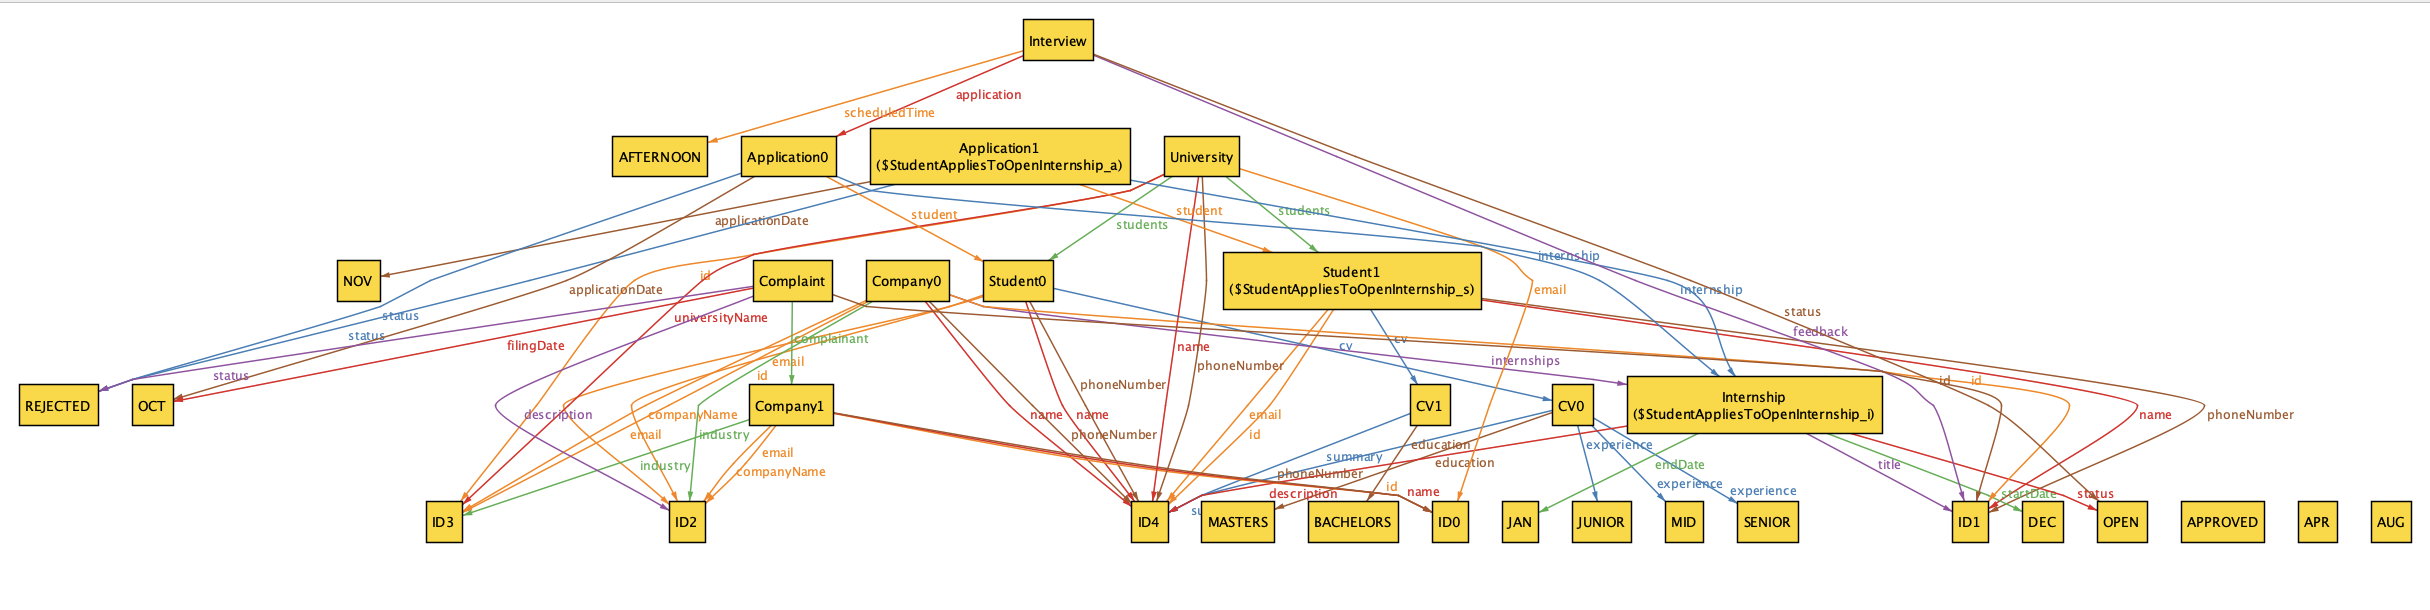
\includegraphics[width=1\linewidth, height=5cm]{JhaBhatiaSharma/Images/Scenario 1.png}
    \caption{Scenario for Student Applies to an \textit{Open Internship}.}
    \label{fig:scenario1}
\end{figure}

%-----------------------------------------
\subsubsection{Scenario: Approved Internship Transition}
\paragraph{Description:} Once an application is \texttt{APPROVED}, the corresponding internship should no longer be \texttt{OPEN}.
\paragraph{Predicate:}
\begin{verbatim}
pred ApprovedInternshipScenario {
    some a: Application |
        a.status = APPROVED
        and a.internship.status != OPEN
}
run ApprovedInternshipScenario for 5
\end{verbatim}
\paragraph{Result:} Successful. The Alloy Analyzer verifies the status transition of internships when an application is approved.


\begin{figure}[H]
    \centering
    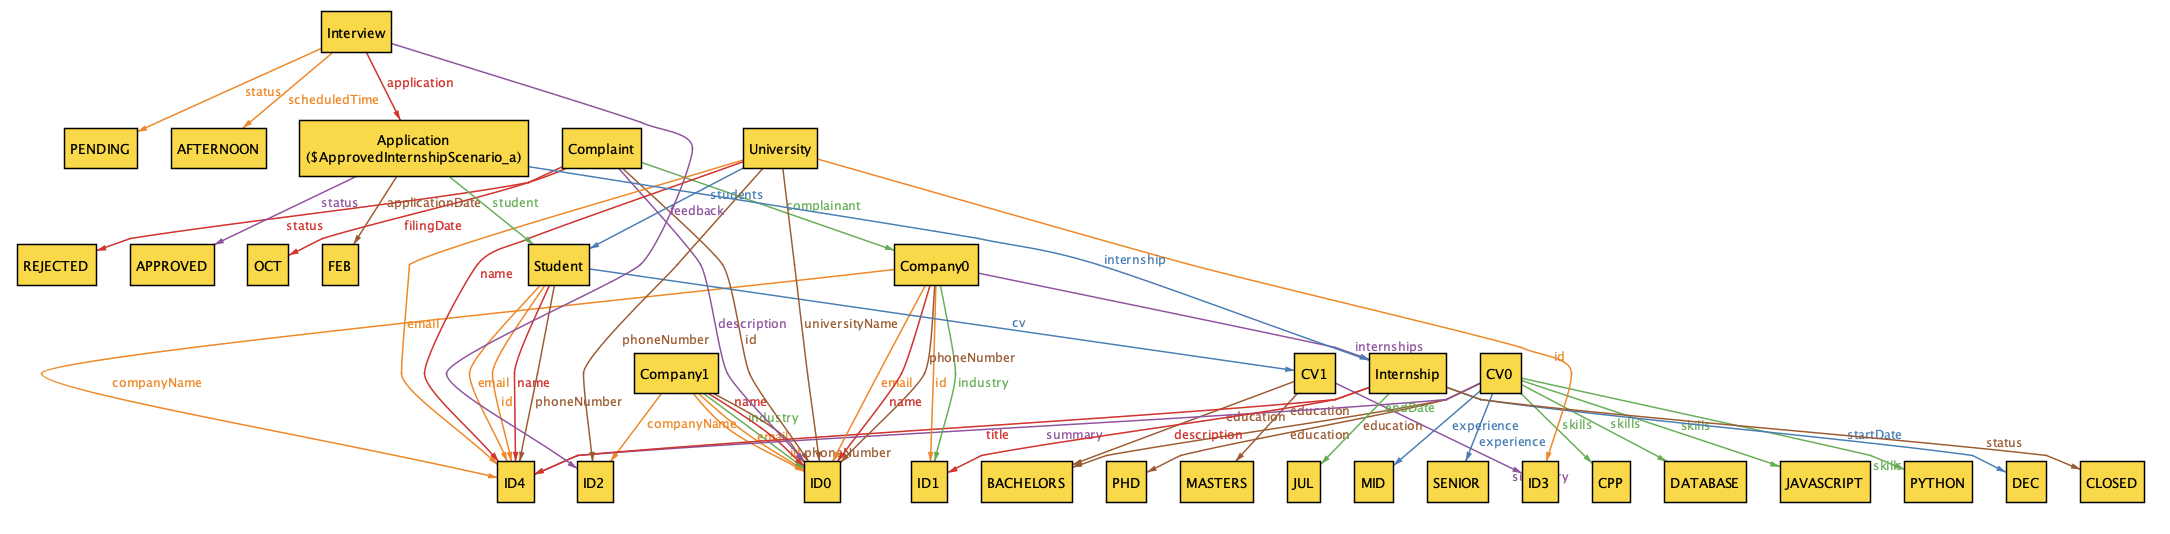
\includegraphics[width=1\linewidth, height=5cm]{JhaBhatiaSharma/Images/Scenario 2.png}
    \caption{Scenario for \textit{Approved Internship}.}
    \label{fig:scenario2}
\end{figure}
%-----------------------------------------
\subsubsection{Scenario: Valid Complaint with Complainant}
\paragraph{Description:} A complaint that is not marked \texttt{REJECTED} must have a valid complainant associated with it.
\paragraph{Predicate:}
\begin{verbatim}
pred ValidComplaintScenario {
    some c: Complaint |
        c.status != REJECTED
}
run ValidComplaintScenario for 5
\end{verbatim}
\paragraph{Result:} Verified. The Alloy Analyzer confirms that all valid complaints are associated with a complainant.


\begin{figure}[H]
    \centering
    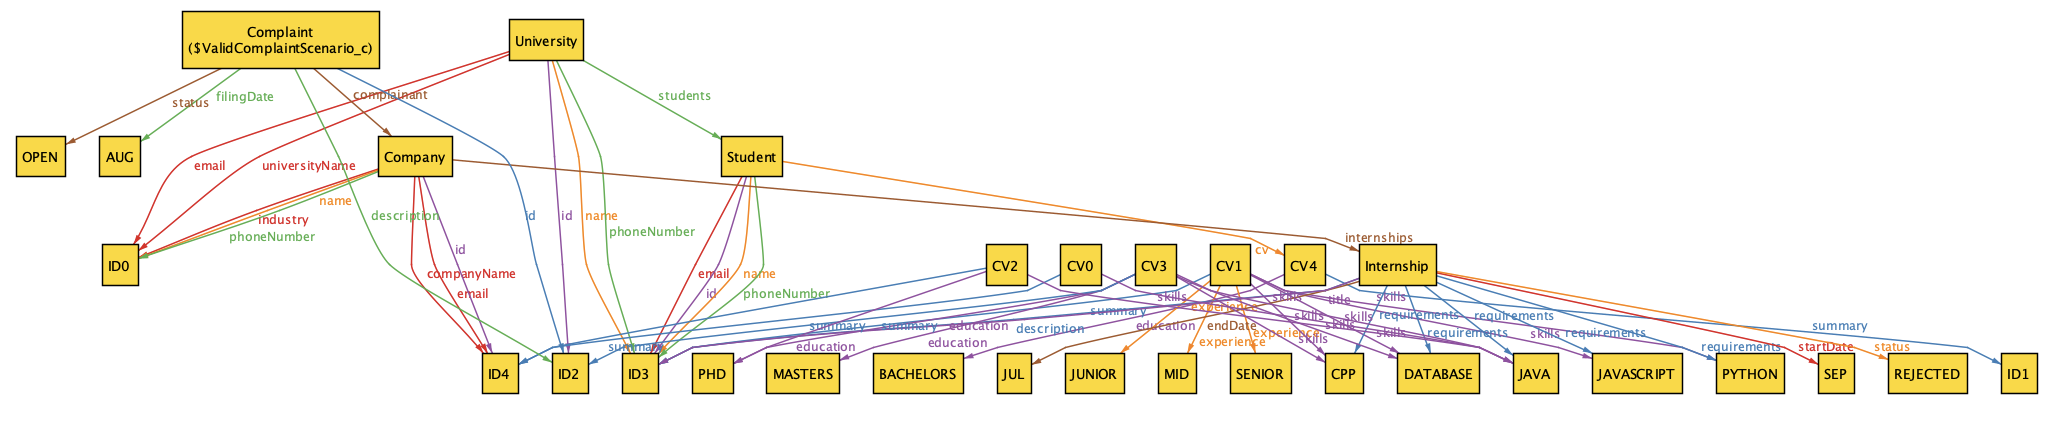
\includegraphics[width=1\linewidth, height=5cm]{JhaBhatiaSharma/Images/Scenario 3.png}
    \caption{Scenario for \textit{Valid Complaint}.}
    \label{fig:scenario3}
\end{figure}

\subsection{Base World for InternHub}
\begin{figure}[H]
    \centering
    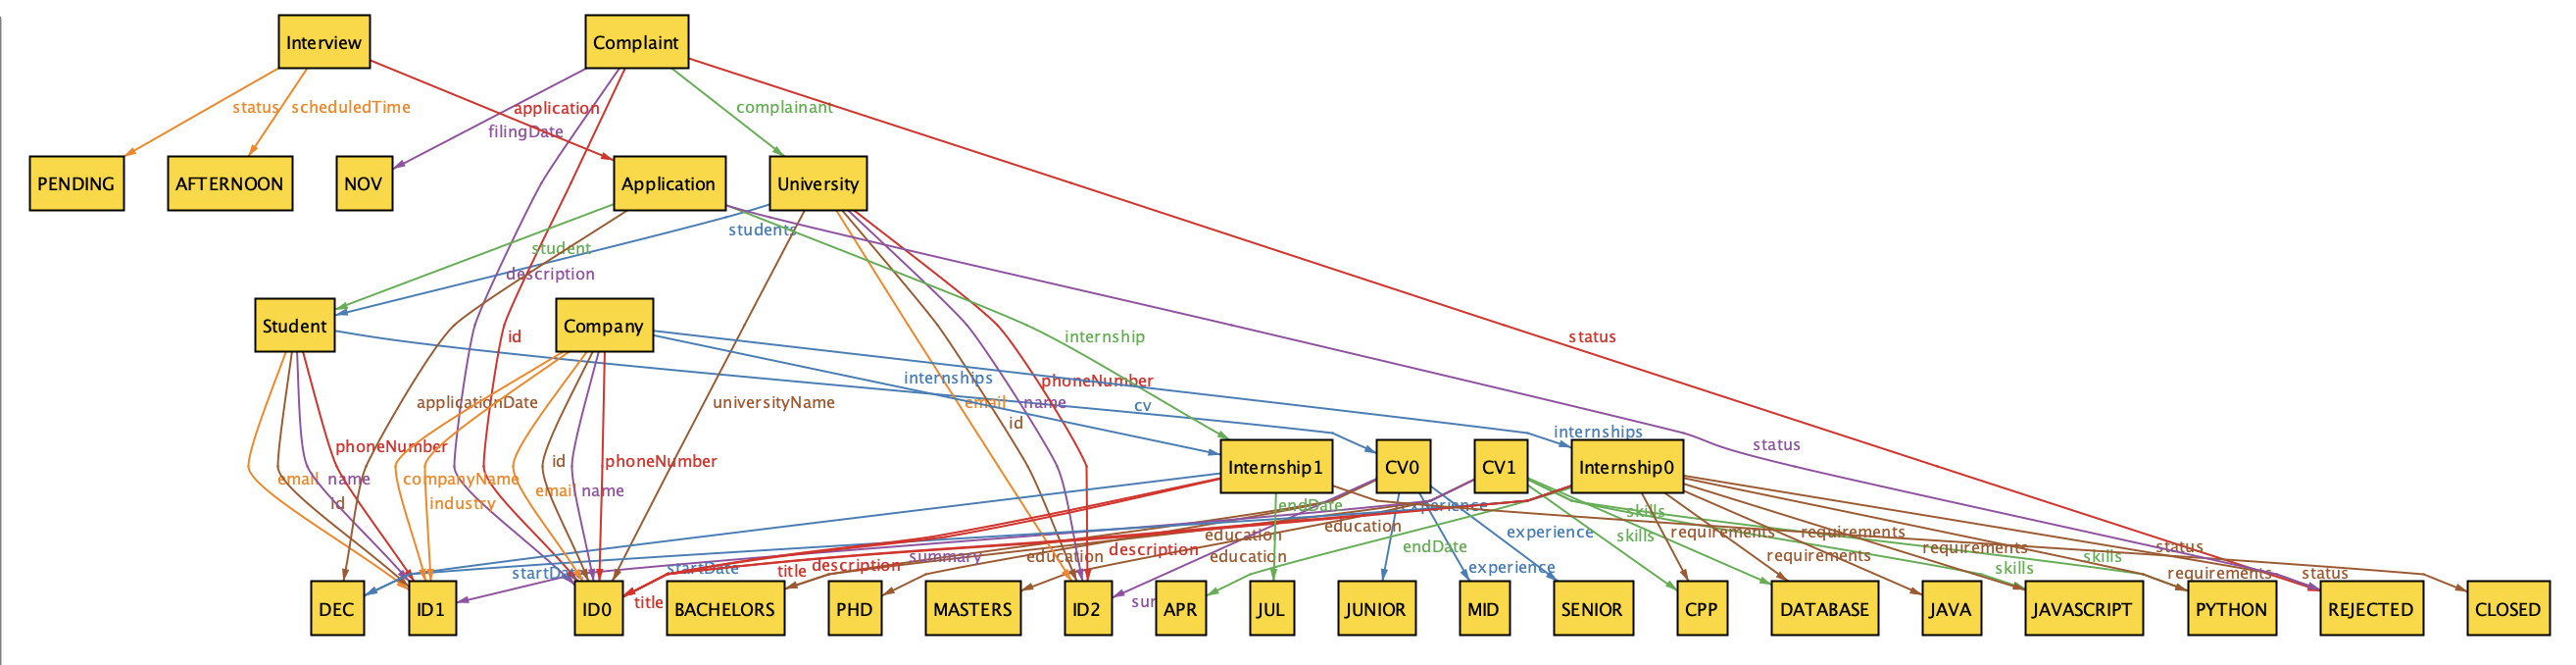
\includegraphics[width=1.2\linewidth]{JhaBhatiaSharma/Images/BaseWorld1.png}
    \caption{Instance for \textit{BaseWorld Simplified}.}
    \label{fig:baseWorld}
\end{figure}

\begin{figure}[H]
    \centering
    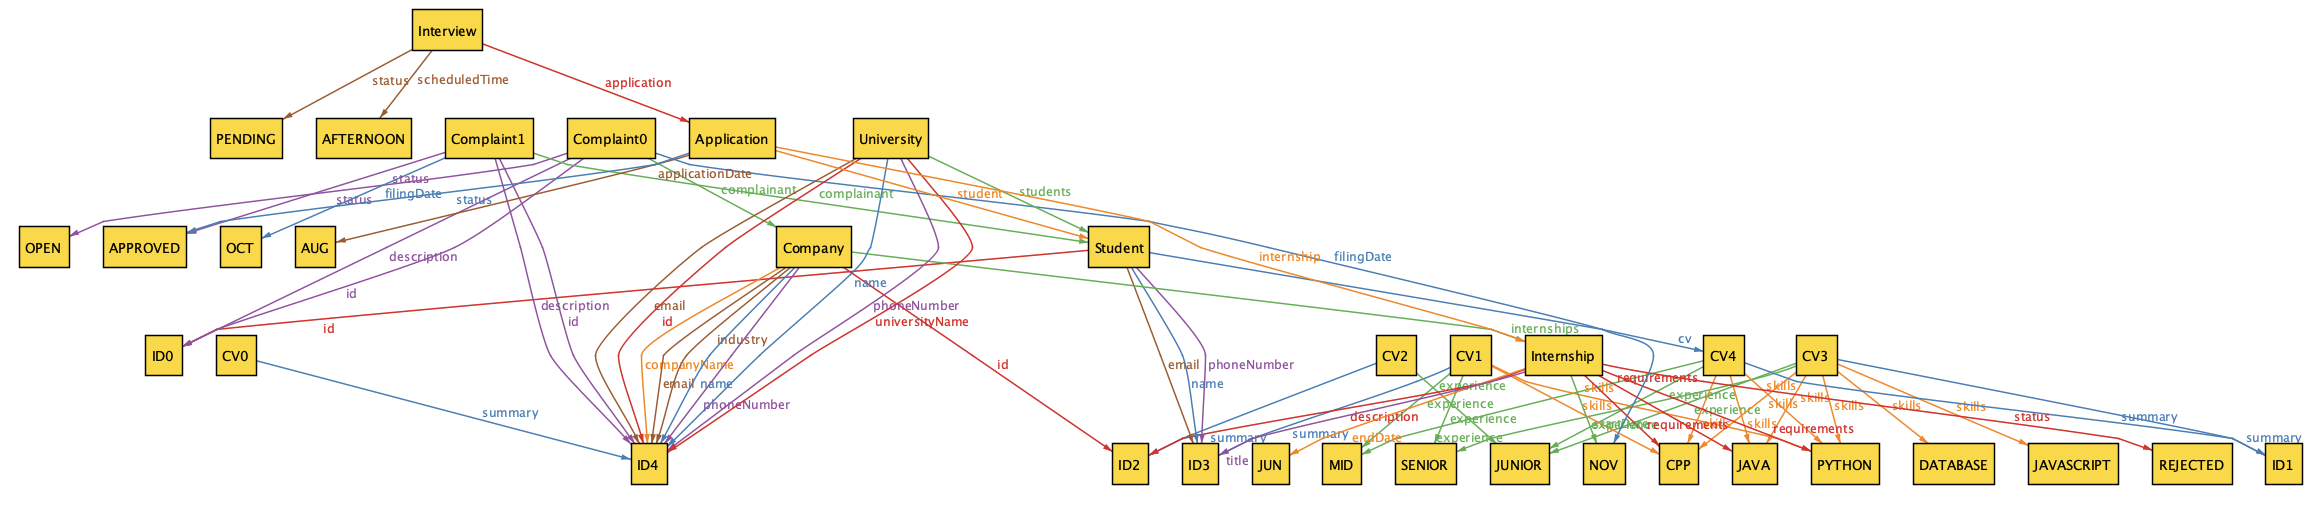
\includegraphics[width=1\linewidth]{JhaBhatiaSharma/Images/BaseWorld2.png}
    \caption{Simplified Instance for \textit{BaseWorld Simplified 2}.}
    \label{fig:baseWorld_magic}
\end{figure}

\begin{figure}[H]
    \centering
    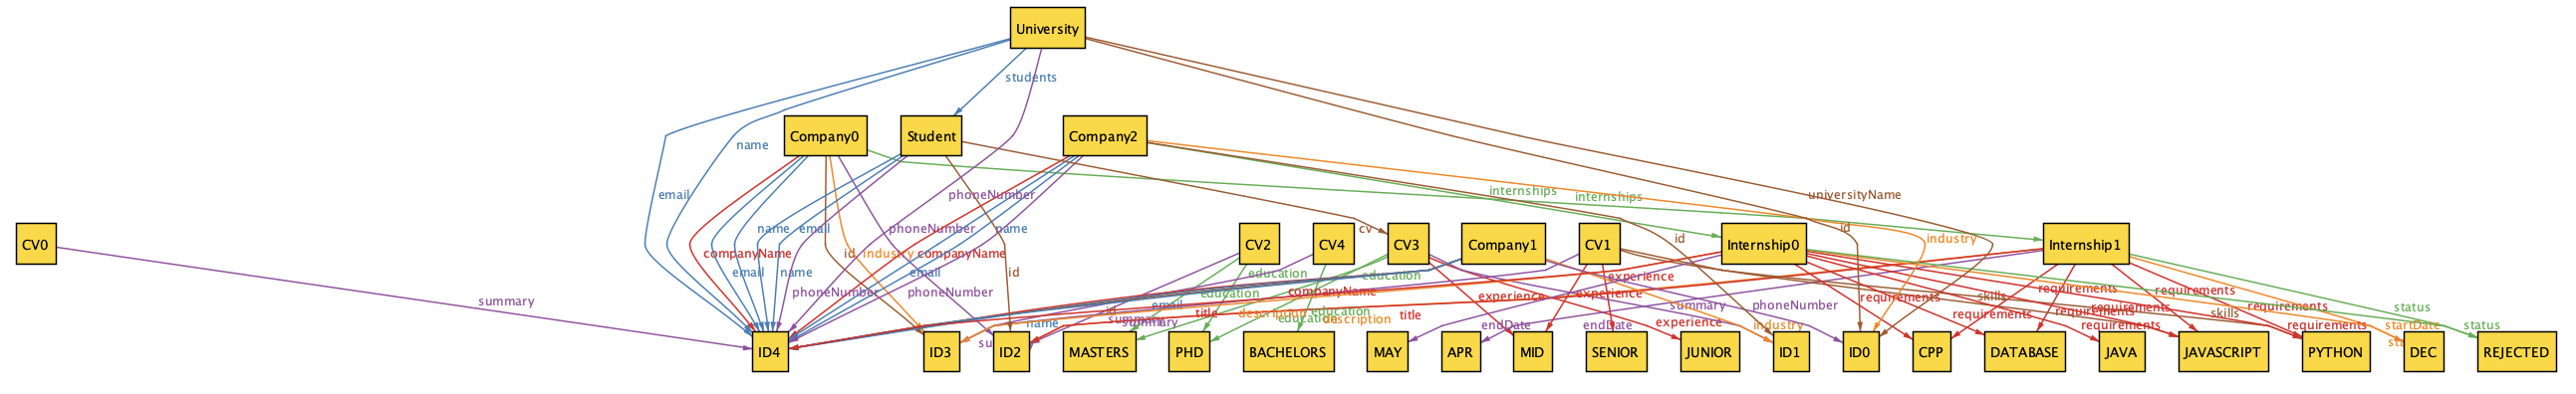
\includegraphics[width=1.12\linewidth]{JhaBhatiaSharma/Images/BaseWorld3.png}
    \caption{Simplified Instance for \textit{BaseWorld Simplified 3}.}
    \label{fig:world_magic}
\end{figure}
